%!TEX root = thesis.tex
\chapter{Discussion}\label{chap:discussion}
\thispagestyle{plain}

    % The discussion is the interpretation and evaluation of the results. It is a
    % comparison of your results with previous findings. It provides the answer to
    % the scientific questions raised in the introduction. It is the "nerve center"
    % of a thesis, whereas the chapter Results may be seen as the "heart".

    % Clearly separate between your own contributions and those of others. Provide
    % rigorous citations of appropriate sources! Explicitly refer to specific 
    % results presented earlier. A certain amount of repetition is necessary. Order
    % discussion items not chronologically but rather logically.

    % The chapter Results answers the question: What has been found? (Facts). The
    % chapter Discussion answers the question: How has the  result to be interpreted?
    % (Opinion).

    % The most important message should appear in the first paragraph. The answer to
    % the key question may appear in the first sentence: e.g., did your original idea
    % work, or didn't it? The following questions may be answered in the discussion
    % section:
    % - Why is the presented method simpler, better, more reliable than previous
    % ones?
    % - What are its strengths and its limitations?
    % - How significant are the results?
    % - How trustworthy are the observations?
    % - Under which conditions and for which region are the results/method valid?
    % - Can the results be easily transferred to other regions or fields?


    It has been shown that the glacier geometry changes simulated by the implemented \vas{} model are conceptually right and suffices as an order of magnitude estimate. However, some important physical processes are not resolved by the \vas{} model, which leads to drastic differences when compared to the flowline model. This should come as no surprise: while the 1.5-dimensional glacier representation of a flowline model is already a strong simplification, the \vas{} model basically simulates a glacier as an inclined brick-shaped block of ice.

    The \vas{} strongly underestimates the initial ice volume when compared to the flowline model, as well as the absolute and relative changes in ice volume. These results are in line with the previously established performances of the scaling approach for estimating glacier ice thickness \citep{Andreassen2015, Farinotti2017}. Similar results for 21st century projections of glacier mass loss are shown by \citet[Figures S1--S20 in the supporting informations]{Marzeion2020}: forced by GCM data with different emission scenarios, the OGGM flowline model predicts a more negative specific mass balance, a stronger area change, a higher mass loss rate and a stronger mass loss for  central Europe as the  original \citet{Marzeion2012b} \vas{} model. All this evidence suggests that the \vas{} is not able to resolve all relevant dynamic processes. Neglecting those processes generally leads to an underestimation of ice volume and its change over time. The absolute value of initial ice volume can be adjusted by using regionally calibrated scaling parameters. However, the sensitivity analysis (Section~\ref{sec:sensitivity_to_scaling_parameters_results}) shows that the relative volume change is not affected by different parameters, which is in line with previous studies \citep{Radic2007, Radic2008}. The missing processes that could be identified in this study are discussed below.

    The positive feedback loop between surface mass balance and surface elevation has a non-negligible effect on glacier mass change \citep{Huss2012a, Schafer2015}. If the surface elevation decreases as a result of a negative mass balance, the air temperature above the ice surface will subsequently increase, according to the negative temperature gradient. Higher temperatures, in turn, lead to increased melt, which further decreases the surface elevation (this feedback loop works analogously for increasing surface elevations due to positive mass balance). However, the only direct feedback between glacier geometry and specific mass balance of the \vas{} model happens at the glacier terminus.
    Changes in glacier length are linearly relayed to changes in terminus elevation, depending on the average surface slope. This is aggravated by the fact that the modeled changes in glacier length are strongly underestimated, which results in a general underestimation of glacier mass change and a symmetric response to positive and negative step changes in temperature. The symmetric response can be reproduced by the flowline model, if the implemented mass-balance-elevation feedback is turned off (see Section~\ref{sec:single_glacier_test_case_results},~\ref{sec:regional_runs_with_all_alpine_glaciers_results}). Additionally, the glacier wide thickness change influences the change of glacier length. \citet{Roe2014} show that glaciers respond to step changes in climate in three overlapping stages:
    \begin{enumerate*}[label=(\arabic*)]
        \item changes in interior thickness cause
        \item changes in terminus flux, which in turn drive
        \item changes in glacier length.
    \end{enumerate*}
    Subsequently, the glacier length does not change exponentially, but much rather sigmoidally. The length change rate needs some time to ramp up to its maximum value, before it slowly drops again and the glacier length approaches its new equilibrium value. The third-order linear ARMA(3,3) model proposed by \citet{Roe2014} is able to adequately simulate all three stages, produces a sigmoidal change of glacier length, and performs comparable to a flowline model.

    % Different results for attribution: Roe et al. (2020) vs Marzeion et al. (2014)
    % Time scales too long
    Using this three-stage model, \citet{Roe2020} attribute all of the observed glacier mass loss over the industrial era to anthropogenic forcings. This disputes the findings of \citet{Marzeion2014a}, who estimated an anthropogenic contribution of only \SI{25\pm35}{\percent} during the period from 1851 to 2010 increasing to \SI{69\pm24}{\percent} over the last twenty years (1991--2000) using the \vas{} model. A possible explanation can be found in the model-internal time scales. The model-internal time scale for length changes used by \citet{Marzeion2012b} is based on the mass turnover $\tau_L \propto 1/P^\text{solid}_\text{clim}(t^*)$ (see Section~\ref{sub:glacier_evolution_model} for details), rather than using the geometric timescale $\tau_L \propto -1/\dot{b}_\text{terminus}$ proposed by \citet{Johannesson1989}. \citet{Roe2020} argue that the computed response times are too large, since the average precipitation is mostly lower than the corresponding terminus ablation rate. This corroborates the findings presented in Section~\ref{sec:sensitivity_to_model_internal_time_scales_results}. The oscillatory behavior of the geometry response can be reduced by lowering the model internal time scales. However, the \vas{} already shows strong short term variability under natural year-to-year climate variability. Lowering the model-internal time scales may result in even stronger fluctuations and make the model react even quicker to changes in climate.

    % An additional argument brought up by \citet{Roe2020} concerns the mass balance calibration method.
    \citet{Roe2020} additionally argue that the mass balance calibration is another source of uncertainty. By assuming that neighboring glaciers are likely in equilibrium around the same time, only climatic factors are considered, while other factors, like the glacier size, are neglected. Small glaciers (or more precisely, glaciers with a short response time) are never far from equilibrium due to their fast geometry adjustments, while large glaciers (or more precisely, glaciers with a long response time) may take many years before they even start reacting to a trend in climate. This potential source of uncertainty is already acknowledged by \citet{Maussion2019}, reasoning that even potentially large errors in \tstar{} will result in comparably small errors in \mustar{}, due to the equilibrium constraint. However, an investigation of this problem is not possible within this study, since the \vas{} model and the OGGM both rely on the same calibration method and are therefore equally affected by it.
    
    % Start area finding problem. TODO: redo and include plots 
    Another potential problem does not concern the model per~se, but the initialization of past glacier states proposed by \citet{Marzeion2012b}. Since the response time scaling introduces a ``glacier memory'', which inhibits to run the model back in time, the value for the initial glacier surface area in 1850 is estimated via an iterative process: iterating over a range of possible values for the 1850 area and choosing the one which results in the area closest to the RGI observation at the year of measurement (see Figure~\ref{fig:start_area:original})\footnote{Implementation note: the task \lstinline`find_start_area()` uses a minimization function rather the proposed iterative process and allows to choose whether to update the terminus elevation or not.}. For each iteration, initial volume and length are estimated from the initial area using the scaling relations. The terminus elevation, however, is not adjusted to the new glacier length, but kept constant at the RGI reference value. Thereby, the new and now larger (or smaller) glacier is confined to the same elevation band as the current one, which implies a lower (or higher) average slope. Intuitively, this may make sense, given the Alpine topography of steep mountains and flatter valleys. However, keeping the initial terminus elevation constant results in equal initial specific mass balance of different sized glaciers, which makes less physical sense. This problem is easily fixed by adjusting the terminus elevation to the new glacier length, in the same way as during all the other time steps. This results in higher and mostly positive values of initial specific mass balance for smaller initial glaciers (given that they retreated into higher elevations), and lower and possibly negative values for larger initial glaciers (given that they reach further into the ablation zone). However, by doing so, the model is not able to reproduce a surface area close to the observed area in 2003 for some glaciers, regardless of the initial area in 1850 (see Figure~\ref{fig:start_area:overturn}). Furthermore, the larger initial glaciers end up with a lower surface area than the smaller initial glaciers. This turn over is also seen for ice volume and glacier length (not shown), and reinforces the notion that the model internal time scales are too long, i.e. past glacier states have too much of an influence. By allowing for instant geometry updates, i.e., setting the time scales to $\tau_L = \tau_A = \SI{1}{\year}$, the ``overturning'' vanishes. However, the areas still converge to a similar range as for the physical consistent model, which may in some cases be far off the observed value (see Figure~\ref{fig:start_area:instant}). When comparing the original and physical consistent implementation, the same initial areas, even if only slightly different from the RGI reference value, result in drastically different glacier evolutions (look at $A_0 = \SI{6.65}{\square\kilo\meter}$ and $A_0 = \SI{10.42}{\square\kilo\meter}$ in Figure~\ref{fig:start_area:original}~and~\subref{fig:start_area:overturn}). It hints on a dependency of the time scales to the average slope. This additionally supports the arguments that the terminus mass balance is a better suited to estimate glacier time scales than precipitation, since it also depends on the average surface slope, or much rather the terminus elevation.

    % Figure showing Hintereisferner time series plots - on page
    \begin{figure}[ht]
      \centering

      % original impelementation
      \begin{subfigure}[b]{0.3\textwidth}
        \caption{Original implementation with constant, i.e., not adjusted initial terminus elevation}
        \label{fig:start_area:original}
        \centering
        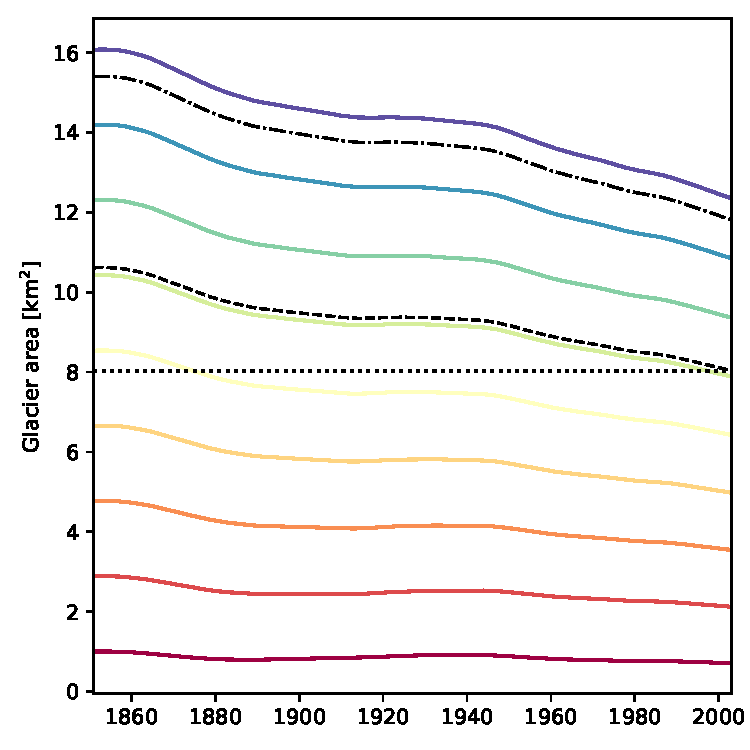
\includegraphics[width=\textwidth]{../plots/start_area/RGI60-11.00897_original.pdf}
      \end{subfigure}
      \hfill
      % my implementation
      \begin{subfigure}[b]{0.3\textwidth}
        \caption{Physical consistent implementation with adjusted initial terminus elevation}
        \label{fig:start_area:overturn}
        \centering
        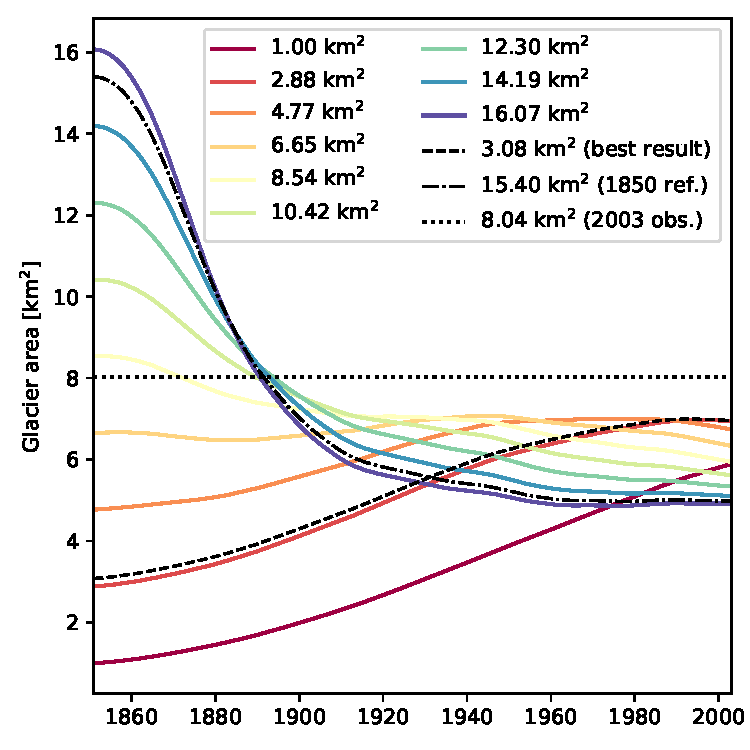
\includegraphics[width=\textwidth]{../plots/start_area/RGI60-11.00897_overturn.pdf}
      \end{subfigure}
      \hfill
      % instant update
      \begin{subfigure}[b]{0.3\textwidth}
        \caption{Physical consistent implementation with added instant geometry changes, i.e., $\tau_L = \tau_A = \SI{1}{\year}$}
        \label{fig:start_area:instant}
        \centering
        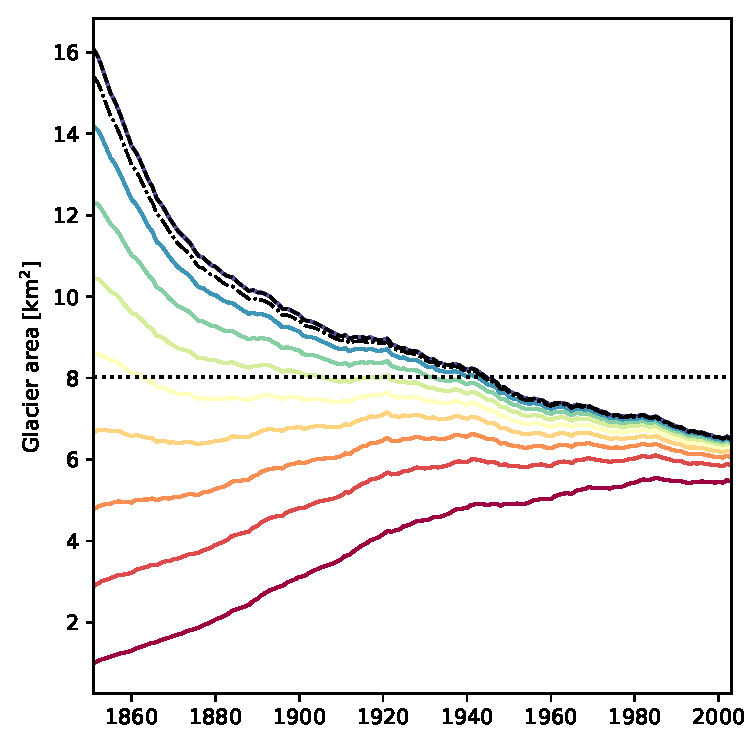
\includegraphics[width=\textwidth]{../plots/start_area/RGI60-11.00897_instant.pdf}
      \end{subfigure}
      
      \caption{Evolution of Hintereisferner (RGI60-11.00897) surface area for different initial values, from 1851 to 2003, forced by HISTALP climate data.}
      \label{fig:start_area}
    \end{figure}

    % Trying to sell the OGGM template module
    As a final note, the implementation of the \vas{} model in the OGGM framework is a success on its own. As suggested by \citet{Maussion2019}, the implementation of simpler approaches, such as the one presented here, allows to test the benefits of the increased model complexity. Such extension of the OGGM are obviously not limited to simple model, but may as well add more complex processes \citep[e.g., an improved calving parametrization,][]{Recinos2019}. It shows the benefits of an open source, modular, community driven glacier model. Comparing different parametrization and estimating uncertainties are imperative to improve projections of future glacier mass loss and its consequences. The comparison shown here is merely a first step.

    % As already mentioned, the here implemented model can be found in its own \href{https://github.com/OGGM/oggm-vas}{GitHub repository}. While the separation from the OGGM codebase complicates continuous testing and ensuring the consistency of the code, it also ensures correct attribution. For details about contributing or extending the OGGM visit the \href{https://docs.oggm.org/en/latest/add-module.html}{documentation}.
